% Autor: Kamil Ziemian

% --------------------------------------------------------------------
% Podstawowe ustawienia i pakiety
% --------------------------------------------------------------------
\RequirePackage[l2tabu, orthodox]{nag}  % Wykrywa przestarzałe i niewłaściwe
% sposoby używania LaTeXa. Więcej jest w l2tabu English version.
\documentclass[a4paper,11pt]{article}
% {rozmiar papieru, rozmiar fontu}[klasa dokumentu]
\usepackage[MeX]{polski}  % Polonizacja LaTeXa, bez niej będzie pracował
% w języku angielskim.
\usepackage[utf8]{inputenc}  % Włączenie kodowania UTF-8, co daje dostęp
% do polskich znaków.
\usepackage{lmodern}  % Wprowadza fonty Latin Modern.
\usepackage[T1]{fontenc}  % Potrzebne do używania fontów Latin Modern.



% ----------------------------
% Podstawowe pakiety (niezwiązane z ustawieniami języka)
% ----------------------------
\usepackage{microtype}  % Twierdzi, że poprawi rozmiar odstępów w tekście.
% \usepackage{graphicx}  % Wprowadza bardzo potrzebne komendy do wstawiania
% grafiki.
% \usepackage{verbatim}  % Poprawia otoczenie VERBATIME.
\usepackage{textcomp}  % Dodaje takie symbole jak stopnie Celsiusa,
% wprowadzane bezpośrednio w tekście.
\usepackage{vmargin}  % Pozwala na prostą kontrolę rozmiaru marginesów,
% za pomocą komend poniżej. Rozmiar odstępów jest mierzony w calach.
% ----------------------------
% MARGINS
% ----------------------------
\setmarginsrb
{ 0.7in} % left margin
{ 0.6in} % top margin
{ 0.7in} % right margin
{ 0.8in} % bottom margin
{  20pt} % head height
{0.25in} % head sep
{   9pt} % foot height
{ 0.3in} % foot sep



% ------------------------------
% Inne użyteczne pakiety
% ------------------------------
\usepackage{csquotes}  % Pozwala w prosty sposób wstawiać cytaty do tekstu.
\usepackage{xcolor}  % Pozwala używać kolorowych czcionek (zapewne dużo
% więcej, ale ja nie potrafię nic o tym powiedzieć).
\usepackage{tikz}  % Pakiet do tworzenia grafiki wektorowej
\usetikzlibrary{positioning, calc, decorations.markings}
% Uaktywnia odpowiednie biblioteki TikZ



% ------------------------------
% Pakiety do tekstów naukowych
% ------------------------------
\let\lll\undefined  % Amsmath gryzie się z językiem pakietami do języka
% polskiego, bo oba definiują komendę \lll. Aby rozwiązać ten problem
% oddefiniowuję tę komendę, ale może tym samym pozbywam się dużego Ł.
\usepackage[intlimits]{amsmath} % Podstawowe wsparcie od American
% Mathematical Society (w skrócie AMS)
\usepackage{amsfonts, amssymb, amscd, amsthm} % Dalsze wsparcie od AMS
\usepackage{siunitx}  % Dla postrzego pisania jednostek fizycznych
\usepackage{upgreek}  % Ładniejsze greckie litery
% Przykładowa składnia: pi = \uppi
\usepackage{slashed}  % Pozwala w prosty sposób pisać slash Feynmana.
\usepackage{calrsfs}  % Zmienia czcionkę kaligraficzną w \mathcal
% na ładniejszą. Może w innych miejscach robi to samo, ale o tym nic
% nie wiem.



% ----------------------------
% Pakiety dla tego konkretnego pliku
% ----------------------------
\usepackage{wasysym}  % Daje symbol uśmiechu.
\usepackage{indentfirst}  % Wcięcie w pierwszym akapicie



% ----------
% Tworzenie otoczeń "Twierdzenie", "Definicja", "Lemat", etc.
\newtheorem{twr}{Twierdzenie} % Komenda wprowadzająca środowisko (?)
% ,,twr'' do pisania twierdzeń matematycznych
\newtheorem{defin}{Definicja} % Analogicznie jak powyżej
\newtheorem{wni}{Wniosek}



% --------------------------------------------------------------------
% Dodatkowe ustawienia dla języka polskiego
% --------------------------------------------------------------------
\renewcommand{\thesection}{\arabic{section}.}
% Kropki po numerach rozdziału (polski zwyczaj topograficzny)
\renewcommand{\thesubsection}{\thesection\arabic{subsection}}
% Brak kropki po numerach podrozdziału



% ----------------------------
% Ustawienia różnych parametrów tekstu
% ----------------------------
\renewcommand{\arraystretch}{1.2}  % Ustawienie szerokości odstępów między
% wierszami w tabelach.





% --------------------------------------------------------------------
% Różne komendy zdefiniowane dla ułatwienia pracy z LaTeXem
% --------------------------------------------------------------------

% ##########
% Definicje odstępów w tekście
\newcommand{\spaceOne}{3em}
\newcommand{\spaceTwo}{2em}
\newcommand{\spaceThree}{1em}
\newcommand{\spaceFour}{0.5em}



% ##########
% Skróty do często używanych komend
\newcommand{\ld}{\ldots}
\newcommand{\tbs}{\textbackslash}  % Backslash w tekście

% ##########
% Podstawowa komendy do edycja tekstu
\newcommand{\tb}{\textbf}
\newcommand{\noi}{\noindent}


\newcommand{\powt}[1]{$t^{ #1 }$}
\newcommand{\pd}[3]{ \frac{ \partial^{ #1 } { #2 } }
  { \partial { #3 }^{ #1 } } }


% Komendy wspomagające wspólną edycję tekstu (JM)
\newcommand{\changed}[1]{\textcolor{yellow}{#1}}
\newcommand{\tothink}[1]{\textcolor{blue}{#1}}
\newcommand{\toadd}[1]{\textcolor{green}{#1}}
\newcommand{\todel}[1]{\underline{\textcolor{red}{{\em{#1}}}}}
\newcommand{\corr}[2]{{{\todel{#1}} }{\toadd{#2}}}

% --------------------------------------------------------------------
% Koniec komend
% --------------------------------------------------------------------



% ----------------------------
% Pakiet "hyperref"
% Polecano by umieszczać go na końcu preambuły.
% ----------------------------
\usepackage{hyperref} % Pozwala tworzyć hiperlinki i zamienia odwołania
% do bibliografii na hiperlinki.





% --------------------------------------------------------------------
\title{Porady do~pisania sprawozdań z~eksperymentów na~pracowni.
  \large Z~uwagami o~korzystaniu z~systemu \LaTeX a}

\author{Kamil Ziemian}
% Pomogli mi
% --------------------------------------------------------------------





% ####################################################################
\begin{document}
% ####################################################################


% ############################
\maketitle
% ############################



% ############################
\section*{O~tym poradniku}
\label{sec:otym}


\begin{itemize}
\item[--] Tekst nie tylko można, ale należy przekazywać dalej, każdemu
  komu może~się on~przydać.

\item[--] W~tekście tym na~pewno~są obecne błędy, będziemy wdzięczni
  za~przesyłanie ich na~adres~mailowy~\tb{kziemianfvt@gmail.com}.
  Można też nanieść poprawki samemu w~egzemplarzu pliku dostępnego
  na~GitHubie i~utworzyć Pull requesta \\
  \href{https://github.com/KZiemian/Various-texts/tree/master/O-pisaniu-sprawozdan-z-LaTeXem}{https://github.com/KZiemian/Various-texts/tree/master/O-pisaniu-sprawozdan-z-LaTeXem}.

\item[--] Wszelkie propozycje zmiany bądź poprawy obecnej wersji można
  kierować do~wyżej podanego maila, bądź na~GitHuba. Postaramy~się
  je~rozpatrzyć i~maksymalnie szybko wprowadzić. Prosimy też
  o~informacje, czy~dana osoba ma~zostać dopisana do~listy autorów.

\item[--] W~podanych przykładach w~trybie matematycznym celowo dawane
  są duże odstępy, aby wzory nie zlewał~się w~jeden nieprzerwany ciąg
  znaków.

\item[--] Przyjęliśmy konwencję ,,komputerową'', by~część ułamkową
  liczb pisać po~kropce (3.14) nie zaś po~przecinku (3,14).

\item[--] Punkt o~nazewnictwie ,,odchylenia
  standardowego''/,,niepewności pomiarowej'' wymaga dopracowania
  i~uściślenia. Jednak jego obecna forma wydaje~się dość praktyczna,
  więc niech na~razie zostanie jak jest.

\item[--] Jeżeli treść jakiegoś punktu wydaje~się tak
  prosta/oczywista, że~nie warto nawet o~tym wspominać, to~zapewne
  została tu~umieszczona, bo~pojawiła~się w~jednym, bądź kilku,
  poprawianych sprawozdaniach poprawionych przez autora tego tekstu,
  bądź osoby które mu~pomagały. Banalne błędy wyglądają zwykle
  najgorzej, dlatego tu przed nimi ostrzegamy i~radzimy jak~je
  eliminować.

\item[--] Staraliśmy~się żeby tekst ten był możliwie poprawny
  merytorycznie oraz~by przedstawiał obecnie obowiązujące konwencje
  i~standardy. Dlatego staraliśmy~się konsultować te~tematy w~których
  nasza wiedza nie jest wystarczając głęboka. Mimo tego pewne
  archaizmy i~błędy mogły pozostać, prosimy więc używać niniejszych
  porad z~rozwagą.

\item[--] Zdania uczonych~są podzielone w~wielu sprawach, wliczając
  w~to standardy pisania sprawozdań i~konwencje. Stąd nawet jeśli
  jakiś punkt w~tym tekście jest napisany zupełnie poprawne, w~zgodzie
  z~tym jak wiele osób to~robi, ktoś może wymagać zupełnie innego
  podejścia do~sprawy.

  Jako przykład można wskazać dyskusję tego, jak należy podawać
  ostateczny wynik eksperymentu.

\item[--] Chcielibyśmy podziękować Karolowi Capale, Wojciechowi Dybie
  i~Janowi Majorowi za~pomoc w~pisaniu tych porad, uzupełnienie ich
  treści oraz~wskazane przez nich błędy i~zaproponowane poprawki. Jak
  również Piotrowi Buremu i Krzysztofowi Musiałowi, za~uważna lekturę
  i~wskazanie wielu błędów.

  Szczególne podziękowania należą~się Markowi Kopciuchowi,
  za~poprawienie część tekstu dotyczącej różnych typów błędów,
  wskazanie wielu przeoczeń i~źle napisanych fragmentów oraz ogólną
  ocenę tekstu.

  Błędy i~niedociągnięcia w~obecnej wersji tekstu~są winą tylko jego
  autorów.
\end{itemize}





% ############################
\section{Podstawowe problemy}
\label{sec:podstawowe}

\begin{itemize}
\item[--] \textbf{Bardzo ważne.} Po skończeniu pisania dowolnego
  tekstu każdy powinien zrobić jedną niezwykle trudną rzecz:
  przeczytać go spokojnie i~uważnie. Doświadczenie wskazuje,
  że~udaje~się to rzadko. Lektura zaś własnej pracy, może przynieść
  wiele momentów zaskoczenia, gdy~odkryjemy co~napisaliśmy.

\item[--] Wszystkie wielkości fizyczne muszą podawać jawnie jednostki
  w~których~są wyrażone\footnote{Chyba, że~jest to wielkość
    bezwymiarowa, np. ilość przebadanych kondensatorów.}!!!

\item[--] Pewnych rzeczy człowiek nie może być pewien, jedną z~nich
  jest to, czy wszystkie wielkości fizyczne wyraził we~właściwych
  jednostkach. Jeśli twój wynik jest absurdalny, po~pierwsze sprawdź
  czy~dobrze przeliczyłeś wszystkie jednostki.

  A~potem sprawdź to~jeszcze dwa razy. Jeśli wynik wciąż jest
  absurdalny, poszukaj innej przyczyny.
\end{itemize}





% ##########
\subsection{Odchylenie standardowe, niepewność, błąd, dokładność
  i~cała reszta bałaganu}
\label{sec:odchylenie}

\begin{enumerate}
\item ,,Błąd pomiaru'', ,,niepewność pomiarowa'', ,,dokładność
  pomiarowa'' i~,,odchylenie standardowe pomiaru'' to wszystko różne
  nazwy na jedno i~to samo\footnote{Z~pewnymi wyjątkami o~których
    będzie później.}! Ponieważ jest strasznie mylące nazywać tę~samą
  wielkość raz ,,dokładnością'', a~raz ,,błędem''\footnote{Osobna
    sprawa, że~jest to iście absurdalny dobór słów!}, dlatego w~tej
  części porad zdecydowaliśmy~się używać neutralnej nazwy ,,odchylenie
  standardowe''.

\item Odchylenie standardowe musi mieć ten sam wymiar jak wielkość
  do~której~się odnosi. Inaczej wszak porównywanie tych liczb nie
  miałoby sensu. Należy zawsze~się upewnić, że~tak w~istocie jest
  i~wszędzie ten wymiar podawać.
  % Np.~jeśli pomiar długości stołu w~daje

\item Odchylenie standardowe wielkości fizycznej~$x$ zapisuje~się
  zwykle jako $\sigma_{ x }$, $\sigma( x )$, $\Delta_{ x }$ , bądź
  $\Delta x$. Zdarzają~się też inne oznaczenia, np.~$u( x )$. Jeśli
  więc mamy długość powiedzmy stołu, oznaczaną~$L$, to jej odchylenie
  standardowe zapiszemy jako $\sigma_{ L }$, $\sigma( L )$,
  $\Delta_{ L }$, $\Delta L$, $u( L )$\footnote{Skrót ,,$u( x )$''
    pochodzi od~angielskiego słowa ,,uncertainty'', czyli
    ,,niepewność''.}.

\item Wedle obecnie przyjętych norm odchylenie standardowo
  zaokrągla~się do~dwóch cyfr znaczących tzn.~zaokrąglamy do dwóch
  cyfr poczynając od~pierwszej różnej od~0. Przykłady znajdują~się
  w~poniższej tabeli.
  \begin{figure}[h]
    \centering
    \begin{tabular}[h]{|r @{.} l |r @{.} l|}
      \hline
      \multicolumn{2}{|c}{Odchylenie standardowe}
      & \multicolumn{2}{|c|}{Po zaokrągleniu} \\
      \hline
      0&0147 & 0&015 \\
      1&24   & 1&2 \\
      124&47 & 120&0 \\
      \hline
    \end{tabular}
    \caption{Jak zaokrąglać odchylenie standardowe.}
    \label{fig:odchylenie}
  \end{figure}

\item Zwykle przyjmuje~się taki wybór jednostek albo sposób zapisu,
  by~odchylenie standardowe nie posiadało części całkowitej.
  Przykładowo odchylenie $1.2 \si{.cm}$ zapisalibyśmy np.~jako
  $0.012 \si{.m}$, zaś~$2.4 \si{.kg}$ jako $0.24 \times 10 \si{.kg}$.

\item Przyjęło~się, że jeśli drugą cyfrą znaczącą odchylenia
  standardowego jest zero to zapisujemy je, pomimo tego, że~nie jest
  to konieczne. Czyli odchylenie~0.2 należy zapisywać jako~0.20.
  Robiąc inaczej moglibyśmy wywołać błędne wrażenie, że~zaokrąglamy
  do~jednej cyfry znaczącej.

\item Wynik należy zaokrąglić do~tego samego miejsca dziesiętnego
  co~jego odchylenie standardowe. Jeśli więc mamy pomiar długości rury
  $L = 1.23189 \si{.m}$ z~niepewnością $\sigma( L ) = 0.012 \si{.m}$,
  to~zaokrąglamy go~do~$L = 1.232 \si{.m}$. \tb{Uwaga!} Przed
  zaokrąglaniem upewnij~się, że~wielkość i~jej odchylenie~są wyrażone
  w~tych samych jednostkach (czyli nigdy nie zaokrąglaj długości
  w~metrach do~odchylenia w~centymetrach).

\item Jeżeli zaokrąglamy liczbę kończącą~się cyfrą 5 np.~47.95, to
  w~celu minimalizacji błędów najlepiej jest stosować jedną
  z~konwencji zaokrąglania. Obecnie najpopularniejszą konwencją jest
  zaokrąglanie do~,,najbliższej liczby parzystej''. \tb{Przykład:}
  jeśli zaokrąglamy 21.5 to~zarówno do~22.0 jak i~21.0 mamy
  ,,odległość'' 0.5, jednak 22.0 jest liczbą parzystą, więc
  zaokrąglamy do~niej. Na tej samej zasadzie 22.5 również zaokrąglamy
  do~22.0. Analogicznie robimy dla części dziesiętnej: 0.475
  zaokrąglamy do~0.48, tak samo jak 0.485. Pewne wytłumaczenie tego
  można znaleźć w~dodatku~A do~tego pliku. \tb{Tylko, że muszę go
    najpierw napisać.}

  O~tym, że~zaokrąglanie nie musi być rzeczą banalną, a~zdania
  uczonych w~kwestii tego jak należy to robić~są podzielone, można~się
  przekonać czytając artykuł na~angielskiej
  \href{https://en.wikipedia.org/wiki/Rounding}{\emph{Wikipedii
      --~Rounding}}. Metoda tu~polecana nosi tam nazwę \emph{Round half
    to~even}.
\end{enumerate}





% ##########
\subsection{Niepewności przypadkowe, błędy systematyczne i~błędy
  grube. Zamieszania ciąg dalszy}
\label{sec:niepewnosci}

Pisząc tą~część opieraliśmy~się głównie na~dwóch źródłach. Po~pierwsze
na~skrypcie Bogusława Kamysa
\href{http://users.uj.edu.pl/\~ufkamys/BK/smop1N\_h.pdf}{\emph{Statystyczne
    Metody Opracowania Pomiarów~I}}, głównie zaś~z~tego co~jest
na~stronach 17--19. Po drugie na~dodatkach do~książki pod
red.~Andrzeja Magiery
\href{http://www.1pf.if.uj.edu.pl/documents/5046939/5227638/skrypt.pdf}{\emph{I~Pracownia
    Fizyczna}}.

\begin{enumerate}
\item Zgodnie z~normą International Standard Organization~(ISO)
  z~1995~roku, należy stosować słowo ,,niepewność'', zaś słowa
  ,,błąd'' używać tylko dla błędów systematycznych i~błędów grubych.
  Pojęcia te będą wyjaśnione dalej. Jak pisaliśmy wyżej,
  zdecydowaliśmy~się używać do~tej pory pojęcia ,,odchylenie
  standardowe'' zamiast ,,niepewności'', ze~względu na~jego
  neutralność znaczeniową, teraz musimy zająć~się tym dokładniej.
  Dalej będziemy korzystali z~tej konwekcji i~pisali
  o~,,niepewności''.

\item Pomimo wprowadzenia tego standardu, wciąż używa~się zamiennie
  słów\footnote{Jak poprzednio, dość obłędny dobór!} ,,niepewność'',
  ,,dokładność'', ,,błąd'',~etc. Należy~więc być gotowym, na~to,
  że~czytając różne teksty, będziemy musieli rozszyfrowywać co w~danym
  kontekście znaczą te~słowa.

\item Niepewności dzielą~się na
  \begin{enumerate}
  \item niepewności przypadkowe (często to prostu ,,niepewności'');
  \item błędy systematyczne;
  \item błędy grube;
  \item niepewność eksperymentu (tu nazwy mogą być dość zróżnicowane).
  \end{enumerate}

\item \textbf{Niepewności przypadkowe} to~te, które wynikają
  z~istnienia słabych, losowych efektów, których \tb{zawsze należy~się
    spodziewać}. Przykładowo, mierzymy temperaturę wrzenia wody,
  ogrzewając ją~palnikiem gazowym. Ze~względu na~losowy ruch powietrza
  płomień~się przemieszcza, woda nie jest ogrzewana równomiernie i~nie
  zaczyna wrzeć cała w~jednym momencie.

  Więcej na~temat niepewności przypadkowych będzie w~części
  \emph{Estymator, estymacja i~inne groźne słowa}
  \eqref{sec:estymator}.

\item \textbf{Błędy systematyczne}, to~błędy ,,wbudowane'' w~sam
  sposób przeprowadzania danego eksperymentu, są~więc popełniane
  systematycznie. Przykładowo, ochładzamy próbkę metalu jednocześnie
  badając jego przewodność elektryczną. Mierzący temperaturę
  termometr może potrzebować więcej czasu niż~próbka,
  aby~zmniejszyć swoją temperaturę, będzie więc systematycznie ją
  zawyżał. Aby~wyeliminować ten problem należałoby powtórzyć pomiar
  przy ogrzewaniu metalu i~porównaniu wyników.

  Innym, zadziwiająco często pojawiającym~się błędem systematycznym,
  jest ten wynikający z~paralaksy. Osoba wykonująca pomiar patrzy~się
  pod kątem na~aparaturę pomiarową, przez co~systematycznie źle
  odczytuje wyniki\footnote{Zapewne błąd ten wynika z~pragnienia
    pewnych ciał do~pozostania w~spoczynku.}

  O~ile opisany powyżej rodzaj błędów systematycznych jest łatwy
  do~zauważenia i~oszacowania, istnieją inne, znacznie trudniejsze
  do~wykrycia i~oszacowanie, przez co~są~dużo groźniejsze. Może~się
  zdarzyć że~efekt fizyczny, na~którym opieramy pomiar, lub~teoria
  na~podstawie której łączymy bezpośrednio zmierzone wielkości
  fizyczne z~poszukiwaną wielkością powoduje np.~systematyczne
  zawyżanie wyników.

  Należy podkreślić, że~błędy systematyczne \tb{nie} muszą być znane
  eksperymentatorom, co jest dużym wyzwaniem przy przeprowadzaniu
  doświadczeń. Przykładowo, w~badanym procesie fizycznym występuje
  zjawisko, które nie zostało wzięte pod uwagę podczas projektowania
  eksperymentu.

\item \textbf{Błędy grube}, to wszystkie sytuacja kiedy
  eksperymentator zrobił coś bardzo źle, albo~aparatura zawiodła.
  Np.~ktoś zmierzył masę próbki, nie zdejmując z~wagi swojego kubka
  z~herbatą; podczas pomiaru doszło do~awarii sieci elektrycznej,
  w~skutek czego napięcie spadło do~$150 \si{.V}$ i~cały pomiar jest
  bezwartościowy. Każdy pomiar obarczony błędem grubym należy usunąć
  z~rozważań\footnote{Chyba, że~ma~się \tb{naprawdę} dobry powód,
    by~go zostawić.}.

  Również błędy grube \textbf{nie} muszą być znane eksperymentatorom.
  Przykładowo w~kodzie programu obsługującym aparaturę znajduje~się
  błąd\footnote{Niestety, kod dużych programów zawsze zawiera jakieś
    błędy, zwykle bardzo małe. Jednak znane~są przypadki, gdy~błędny
    kod postawiły całe lata badań pod znakiem zapytania.}, który
  błędnie przypisuje wartości pewnym mierzonym wielkościom. Z~tego
  powodu naprawdę ważne wielkości mierzy~się w~kilku niezależnych
  eksperymentach, najlepiej za~pomocą różnych zjawisk fizycznych.

\item \textbf{Niepewność eksperymentu} to~ostateczna niepewność całego
  eksperymentu, musi więc uwzględniać wszystkie poprzednie typy
  niepewności i~błędu.

  W~najprostszym przypadku, gdy usuniemy z~rozważań wszystkie pomiary
  obarczone błędem grubym, niepewność przypadkową oznaczymy
  $\sigma( x )$, niepewność systematyczną przez
  $\Delta_{ \textrm{sys} } x$, wówczas niepewność eksperymentu
  $\sigma_{ \textrm{eks} }( x )$ wynosi (zobacz
  \href{http://www.1pf.if.uj.edu.pl/documents/5046939/5227638/skrypt.pdf}{\emph{I~Pracownia
      Fizyczna}}, wzór~(A.1.6), strona~254)
  \begin{equation}
    \label{eq:1}
    \sigma_{ \textrm{eks} }( x ) = \sigma( x ) + \Delta_{ \textrm{s} } x.
  \end{equation}

  Dobrą zasadą jest to, że~jeśli nie wiesz jak obliczyć pełną
  niepewność eksperymentu (ewentualnie serii pomiarów), należy użyć
  tego wzoru powyżej. Jest jednak od~tego pewien wyjątek, o~którym
  jest mowa w~następnym punkcie.

\item Załóżmy, że~nie jesteśmy w~stanie obliczyć niepewności
  przypadkowej (jej obliczaniu jest poświęcony jest podparagrafa
  \eqref{sec:obliczanie}). Przyczyna może być taka, że~np.~mierzy
  długość małej płytki linijką i~jej najmniejsza przedziałka jest na
  tyle duża, że~wszystkie wyniki~się w~niej mieszczą. Inny przypadek
  jest taki, że~z~jakiegoś powodu wykonaliśmy tylko jeden pomiar danej
  wielkości.

  Wówczas postępujemy w~następujący sposób. Szukamy najmniejszego
  przedziału jaki zawiera wszystkie wyniki, jaki jesteśmy przy użyciu
  dostępnych przyrządów zmierzyć i~oznaczmy jego długość $L$.
  W~przykładzie z~linijką długość ta~będzie równa jej najmniejszej
  podziałce. W~przypadku jeśli wykonaliśmy tylko jeden pomiar, za~$L$
  należy przyjąć długość przedziału w~którym musiał znajdować~się
  prawdziwy wynik, aby~przyrząd wskazał otrzymaną wielkość.
  Przykładowo zmierzyliśmy wartość temperatury
  $T = 10.0$\textcelsius, zaś aparatura pozwala mierzyć~ją
  z~dokładnością do~$0.1$\textcelsius, więc prawdziwa temperatura
  musi zawierać~się w~przedziale
  $9.9$\textcelsius$ - 10.1$\textcelsius. W~tym przypadku mamy
  więc~$L = 0.2$\textcelsius.

  W~obu tych sytuacjach całemu pomiarowi przypisujemy niepewność
  przypadkową
  \begin{equation}
    \label{eq:2}
    \sigma( x ) = \frac{ L }{ 2 \sqrt{ 3 } }.
  \end{equation}
  Uzasadnienie i~wyprowadzenie tego ,,magicznego'' wzoru można znaleźć
  w~\href{http://users.uj.edu.pl/\~ufkamys/BK/smop1N\_h.pdf}{skrypcie}
  Bogusława Kamysa na~stronach~25--26.

\item Pewne błędy mogą być zarówno systematyczne jak
  i~grube\footnote{Czytelnik mógł to już zauważyć po~przytoczonych
    przykładach.}. Na~przykład, jeśli eksperymentator źle skalibrował
  wagę, tak~że zawyża ona o~stałą wartość wagę mierzonych próbek.
  W~takich niejasnych sytuacjach nie należy~się specjalnie przejmować
  pedantyczną klasyfikacją błędów.

\item W~pewnych sytuacjach jest szansa na~usunięcie błędów grubych.
  Weźmy poprzedni przykład ze~źle skalibrowaną wagą. Jeśli jest pewne,
  że~waga cały czas zawyżała wyniki o~stałą wartość, można ją odjąć od
  uzyskanych wyników i~wpleść to~zagadnienie do~sprawozdania, jako
  kalibrację przyrządów pomiarowych.

  \textbf{Podkreślamy}, że~można tak zrobić \textbf{tylko wtedy}, gdy
  jesteśmy pewni, że~to przesunięcie było stałe w~całym eksperymencie
  lub~wykonamy dodatkowo krzywą kalibracyjną dla tej wagi. Krzywą taką
  trzeba dołączyć do~sprawozdania.
\end{enumerate}





% ##########
\subsection{Estymator, estymacja i~inne groźne słowa}
\label{sec:estymator}

Rozpatrzmy następujący przykład\footnote{Ponieważ chcemy by~ten tekst
  był możliwie prosty i~zrozumiały, nie~będziemy tu~omawiali różnych
  niuansów jakie mogą występować w~rzeczywistej sytuacji pomiarowej,
  ani~rozważali bardzo dokładnie matematycznego sensu używanych
  wielkości.}. Chcemy zmierzyć temperaturę wrzenia pewnej cieczy przy
zadanym ciśnieniu. Mierzymy~ją, powiedzmy, 10~razy i~mamy 10~różnych
wyników. Powstaje problem, jak~na~podstawie tych 10~różnych wyników
oszacować wartość temperatury wrzenia występującą w~przyrodzie?
Gdybyśmy mieli dwa wyniki, powiedzmy 93\textcelsius{}
i~94\textcelsius, to~całkiem naturalne byłoby przyjęcie, że~lepiej niż
wybrać jeden z~tych wyników, będzie obliczyć ich średnią
arytmetyczną:~93.5\textcelsius.

Jest to~dość typowy problem: mamy pewną ilość pomiarów i~chcemy na~jej
podstawie oszacować ile wynosi wartość prawdziwa. Funkcję, która
pozwala nam wyliczyć to~oszacowanie nazywamy \emph{estymatorem},
zaś~sam proces szukania takiej wartości \emph{estymacją}. Typowym
sposobem szacowania prawdziwej wielkości na~podstawie $n$~pomiarów
z~których każdy ma~taką samą niepewność przypadkową jest wzięcie
średniej arytmetycznej\footnote{Dla tej wielkości bywa też używane
  oznaczenie $x_{ \textrm{E} }$.}
\begin{equation}
  \label{eq:3}
  \overline{ x } = f( x_{ 1 }, x_{ 2 }, \ld, x_{ n } )
  = \frac{ 1 }{ n } \sum_{ i = 1 }^{ n } x_{ i }.
\end{equation}
Z~sytuacją taką mamy do czynieniach choćby wtedy, gdy wykonujemy tym
samym przyrządem serię pomiarów w~takich samych warunkach.
\textbf{Nigdy} nie można tego wzoru używać, dla~zbioru wyników
o~różnej niepewności. Widzimy\footnote{Mamy nadzieję, że~to prawda.}
na~tym przykładzie, że~estymator jest funkcją, która na~podstawie
$n$~pomiarów zwraca nam~oszacowanie prawdziwej wartości danej
wielkości. Przykłady innych oszacowań prawdziwej wielkości, czyli
estymatorów, podamy dalej.

Chcielibyśmy by~nasze oszacowanie było najlepszym jakie można osiągnąć
dysponując taką ilością wyników. Jednak pytanie ,,Jakie oszacowanie
jest najlepsze?'' (czyli ,,Który estymator jest najlepszy?'')
okazuje~się wcale niebanalne. Dlatego dla jednej wielkości mogą
istnieć różne estymatory o~różnych własnościach i~do~analizy
wybiera~się ten o~najbardziej pożądanych w~danym eksperymencie
cechach. Nie będziemy~się jednak w~ten temat zagłębiać.





% ##########
\subsection{Obliczanie odchylenia standardowego i~związany z~tym
  chaos}
\label{sec:obliczanie}

Zajmijmy~się znów problemem niepewności przypadkowych. Zwykle
oczekujemy, że~są konsekwencją dużej liczy~\tb{niezależnych} czynników
losowych, przy czym wpływ każdego z~nich z~osobna jest bardzo mały.
Choćby takich, że~palnik podgrzewający próbkę nie działa równo,
w~sieci elektrycznej są drobne skoki napięcia, ciśnienie powietrza~się
lekko zmienia, etc. W~takim wypadku centralne twierdzenie graniczne
z~teorii prawdopodobieństwa mówi nam, że~należy~się spodziewać,
iż~wyniki pomiaru, oznaczmy go~$x$, są~opisywane rozkładem
Gaussa\footnote{Nie będziemy tu wchodzić bardziej w~teorię
  prawdopodobieństwa, te rozważania są tylko po~to by uzasadnić
  to~co~jest dalej.}
\begin{equation}
  \label{eq:4}
  f( x ) = \frac{ 1 }{ \sqrt{ 2 \pi } \sigma }
  e^{ \frac{ -( x - x_{ \mathrm{fiz} } )^{ 2 } }{ 2 \sigma^{ 2 } } }.
\end{equation}
$x_{ \textrm{fiz} }$ oznacza wielkość występującą w~przyrodzie, zaś
$\sigma$ jest jej odchyleniem standardowym. Sens jego jest
następujący. Jeśli wykonamy pomiar wielkości danej takim rozkładem
to~z~prawdopodobieństwem około 68.2\% dostaniemy wynik z~przedziału
$[ x_{ \textrm{fiz} } - \sigma,\, x_{ \textrm{fiz} } + \sigma ]$. Dla
pomiaru z~przedziału
$[ x_{ \textrm{fiz} } - 2\sigma,\, x_{ \textrm{fiz} } + 2\sigma ]$
prawdopodobieństwo jego uzyskania wyniesie około 95.5\%.

Załóżmy, że~w~naszym pomiarze bierzemy pod uwagę tylko niepewności
przypadkowe, więc jest on rozpisywany rozkładem Gaussa, i~wykonaliśmy
$n$~pomiarów. Wówczas dobrym estymatorem (oszacowaniem) wartości
występującej w~przyrodzie $x_{ \textrm{fiz} }$ jest średnia
arytmetyczna tych pomiarów, oznaczać ją będziemy przez~$\overline{x}$.
Jeśli~zaś chodzi o~estymator odchylenia standardowego $\sigma$,
to~musimy rozróżnić dwie wielkości.

\begin{enumerate}
\item \tb{Odchylenie standardowe (pojedynczego) pomiaru.} Rozważmy
  jeden z~naszych $n$~punktów pomiarowych~$x_{ i }$. Przez jego
  odchylenie standardowe rozumiemy taką wielkość
  $\sigma_{ \textrm{pom} }( x )$, że~$x_{ \textrm{fiz} }$ znajduje~się
  w~przedziale
  $[ x_{ i } - \sigma_{ \textrm{pom} }( x ),\, x_{ i } + \sigma_{
    \textrm{pom} }( x ) ]$. Wielkość $\sigma_{ \textrm{pom} }$
  estymujemy na~podstawie znajomości wszystkich $n$~pomiarów za pomocą
  wzoru. Najpopularniejszy znany nam estymator tej wielkości to
  \begin{equation}
    \label{eq:5}
    \sigma_{ \textrm{est} }( x )
    = \sqrt{ \frac{ 1 }{ n - 1 }
      \sum_{ i = 1 }^{ n } ( x - \overline{x} )^{ 2 } }.
  \end{equation}
  gdzie $\bar x$ jest estymatorem rzeczywistej wartości wielkości~$x$,
  np.~średnią arytmetyczną wyników pomiarów.

\item \tb{Odchylenie standardowe średniej pomiarów}
  $\sigma_{ \textrm{est} }( \overline{x} )$ to~taka wielkość,
  że~rzeczywista wartość $x_{ \textrm{fiz} }$ zawiera~się w~przedziale
  $[ \overline{x} - \sigma_{ \textrm{est} }( \overline{x} ),\,
  \overline{x} + \sigma_{ \textrm{est} }( \overline{x} ) ]$
  z~prawdopodobieństwem około 68.2\%.

  Związek między niepewnością pomiaru, a~niepewnością średniej
  pomiarów jest bardzo prosty
  \begin{equation}
    \label{eq:6}
    \sigma_{ \textrm{est} }( \overline{x} )
    = \frac{ \sigma_{ \textrm{est} }( x ) }{ \sqrt{ n } },
  \end{equation}
  czyli najpopularniejszy znany nam estymator odchylenia standardowego
  średniej ma~postać
  \begin{equation}
    \label{eq:7}
    \sigma_{ \textrm{est} }( \overline{x} ) = \sqrt{ \frac{ 1 }{ n ( n - 1 ) }
      \sum_{ i = 1 }^{ n } ( x - \overline{x} )^{ 2 } }.
  \end{equation}
\end{enumerate}
\tb{Ważne 1.} Nie wdając~się w~subtelne dywagacje, można podać
następującą prostą regułę. Jako wynik konkretnego eksperymentu
(ewentualnie serii pomiarowej) należy podać średnią arytmetyczną
wyników, zaś~jej niepewność przypadkowa dana jest wzorem \eqref{eq:7}. \\
\tb{Ważne 2.} Jakość estymacji (oszacowania) danej wielkości bardzo
silnie zależy od~ilości pomiarów. Popularne powiedzenie mówi,
że~statystka zaczyna~się od~trzech pomiarów. Czyli dopiero z~trzem
lub~większą liczbą pomiarów jest sens liczyć średnią arytmetyczną,
odchylenie standardowe,~etc. Jeśli chodzi o~ilość pomiarów jaka
uchodzi za wystarczającą, zwykle uważa~się, że~więcej niż~30
lub~więcej niż~100. Jednak podczas zajęć laboratoryjnych często
zupełnie wystarczy 10~wyników.

\toadd{Wytłumaczenie o co chodzi z współczynnikami Student-Fishera.}
Jeśli ma~się za małą ilość pomiarów, aby analiza była wartościowa,
to~zawsze najlepszym rozwiązaniem jest wykonać ich~więcej. Jeśli
jednak nie jest to możliwe, można skorzystać z~metody
\textbf{współczynników Studenta\dywiz Fishera}.





% ##########
\subsection{Jak zapisać wynik pomiaru, czyli o~niebanalności rzeczy
  oczywistych}

Ten fragment bazuje na~stronach 24--25 skryptu
\href{http://users.uj.edu.pl/\~ufkamys/BK/smop1N\_h.pdf}{\emph{Statystyczne
    Metody Opracowań Pomiarów~I}}.

Niech $\overline{x} = 1.3347 \si{.m}$ oznacza estymator długości
jakiegoś obiektu, zaś $\sigma( \overline{x} ) = 0.015322 \si{.m}$
estymator całkowitej niepewności eksperymentu, który omawialiśmy
w~\eqref{sec:niepewnosci}. Po~pierwsze musimy zaokrąglić niepewność
do~dwóch cyfr znaczących, czyli
do~$\sigma( \overline{x} ) = 0.015 \si{.m}$. Teraz zaokrąglamy
estymator długość do~tego samego miejsca dziesiątego co~niepewność:
$\overline{x} = 1.335 \si{.m}$. Polecane~są dwa sposoby zapisu wyniku
z~taką niepewnością.
\begin{enumerate}
\item \tb{Zalecany.} Po~wypisaniu wyniku podajemy w~nawiasie dwie
  cyfry reprezentujące niepewność, następnie zaś~odpowiednie jednostki
  fizyczne danej wielkości. Podany wyżej przykład zapisujemy więc jako
  \begin{equation}
    \label{eq:8}
    x = 1.335(15) \si{.m},
  \end{equation}
  ewentualnie
  \begin{equation}
    \label{eq:9}
    x = 1.335(0.015) \si{.m}.
  \end{equation}
  Sens tego zapisu jest następujący. Przedział
  \begin{equation}
    \label{eq:10}
    [ 1.335 \si{.m} - 0.015 \si{.m},\, 1.335 \si{.m} + 0.015 \si{.m} ]
    = [ 1.320 \si{.m},\, 1.340 \si{.m} ]
  \end{equation}
  zawiera wartość prawdziwą z~prawdopodobieństwem około 68.2\%.
\item W~tym przypadku używamy \emph{rozszerzonej niepewności
    eksperymentu} danej wzorem\footnote{Skrót ,,$U( x )$'' pochodzi
    od~angielskiego słowa ,,uncertainty''.}
  \begin{equation}
    \label{eq:11}
    U( x ) = k \sigma( \overline{ x } ), \quad 2 \leq k \leq 3.
  \end{equation}
  Wynik należy wtedy zapiać jako
  \begin{equation}
    \label{eq:12}
    x = \overline{x} \pm U( x )\: [\textrm{jednostka}],\,
    k = \textrm{przyjęta wartość}.
  \end{equation}
  Niekoniecznie trzeba podawać wartość współczynnika~$k$ w~tej samej
  linii co~wynik, jednak by~uniknąć nieporozumień, stosując ten zapis
  należy \tb{zawsze} umieścić gdzieś w~tekście stwierdzenie,
  że~używa~się rozszerzonej niepewności i~podać użytą do~jej
  obliczania wartość~$k$.

  Stosując dla~poprzedniego przykładu niepewność rozszerzoną z~$k = 2$
  zapisalibyśmy wynik jako
  \begin{equation}
    \label{eq:13}
    x = 1.335 \pm 0.030 \si{.m}.
  \end{equation}
  Sens tego jest następujący. Przedział
  \begin{equation}
    \label{eq:14}
    [ 1.335 \si{.m} - 0.030 \si{.m},\, 1.335 \si{.m} + 0.030 \si{.m} ]
    = [ 1.305 \si{.m},\, 1.365 \si{.m} ]
  \end{equation}
  zawiera wartość prawdziwą z~prawdopodobieństwem około 95.5\%.

  Wszystkie wyżej wymienione wielkości procentowe wynikają z~własności
  matematycznych rozkładu Gaussa\footnote{Tutaj parę rzeczy opisaliśmy
    zbyt skrótowo. Może kiedyś napiszemy to lepiej.}
  (zob.~\eqref{sec:obliczanie}). Prawdopodobieństwo znalezienia
  w~przedziale wartości prawdziwej, dla~dowolnego parametru~$k$, można
  otrzymać obliczając ją~samemu na~podstawie tego rozkładu
  albo~odczytać z~odpowiednich
  \href{https://en.wikipedia.org/wiki/Standard_normal_table}{tablic}.
\end{enumerate}





% ############################
\section{\LaTeX}


% ##########
\subsection{Różne informacje i~porady}

\begin{enumerate}
\item Istnieje wiele edytorów dedykowanych do~\LaTeX a, takich choćby
  jak \TeX Maker, jednak można również używać go~online dzięki stronom
  takim jak \href{https://www.overleaf.com/}{Overleaf}. Jeśli
  zaczynasz swoją znajomość z~\LaTeX em polecamy przyjrzeć~się tym
  edytorom internetowym.

\item \LaTeX{} jest stworzoną przez
  \href{https://en.wikipedia.org/wiki/Leslie_Lamport}{Lesliego
    Lamporta} nakładką na~\TeX a, który z~kolei został stworzony przez
  \href{https://en.wikipedia.org/wiki/Donald_Knuth}{Donalda
    E.~Knutha}. Niektórzy wymawiają go ,,latech'' inni, zaś
  ,,lateks'', jednak jako, że~sam Donald Knuth nie wie która
  \href{https://www.youtube.com/watch?v=8HuwiBPLV3A}{wymowa jest
    poprawna}, nie będziemy~się nad tym problemem rozwodzili, sami
  preferujemy jednak pierwszy wariant.

\item Możliwości \LaTeX a są~trudne do~pojęcia i~nawet po~latach pracy
  potrafi on~zaskoczyć tym co~oferuje i~w~tych poradach tak naprawdę
  tylko zahaczymy o~niego tam gdzie wydaje~się nam to~niezbędne/bardzo
  potrzebne. Zachęcamy jednak do~wygoogolwanie tego co~może on~zrobić,
  zaś~źródła do~nauki które uważamy za~dobre można znaleźć
  w~bibliografii na~końcu tych porad.

  Czemu bowiem nie spróbować pisać za~pomocą hieroglifów?

\item Aspektem \LaTeX a o~którym według nas mówi~się za rzadko, jest
  możliwość tworzenia w~nim rozbudowanej grafiki
  wektorowej\footnote{W~temat tego czym jest grafika wektorowa, nie
    będziemy tu~wchodzili.}. \LaTeX{} ma wbudowane w~siebie dość
  ograniczone możliwości tworzenia takiej grafiki, dlatego warto~się
  zapoznać~się pakietem\footnote{PGF = Portable Graphics Format.}
  \texttt{PGF/TikZ} (często określanym po prostu jako \texttt{TikZ}),
  przykład jego możliwości można zobaczyć na
  rysunku~\eqref{fig:Przyklad} Ma~on ogromne możliwości, jednak jest
  też wymaga wiele od~użytkownika i~często wymaga wejścia naprawdę
  głęboko w~trzewia \LaTeX a.

  Warto zauważyć, że~obecnie można często ominąć potrzebę pisania
  konkretnego kodu \texttt{PGF/TikZa}, zamiast tego można skorzystać
  z~narzędzi takich jak internetowy edytor
  \href{https://www.mathcha.io/}{Mathcha}, które udostępniają
  narzędzia graficzne do~tworzenia rysunków, następnie zaś pozwalają
  eksportować je do~odpowiednich plików, lub~wygenerować kod tworzący
  takie rysunki w~\LaTeX u, .
  
  Materiały na~temat pakietu \texttt{PGF/TikZ} można znaleźć
  w~bibliografii na~końcu tych porad.
\end{enumerate}

\begin{figure}
  \centering

  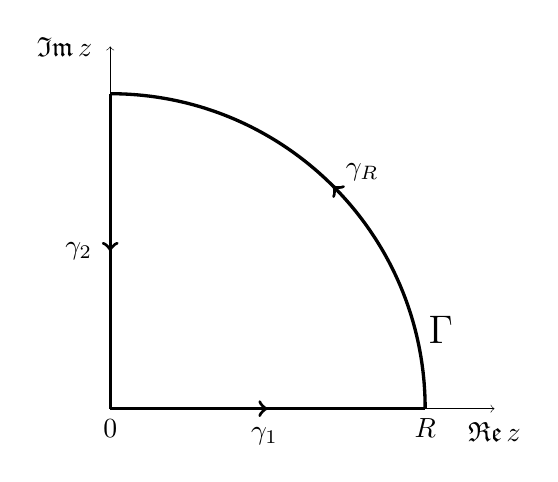
\begin{tikzpicture}
    \def\radius{4}

    % Axes
    \draw[help lines, black, ->] (0, 0) -- (1.22 * \radius, 0);
    \draw[help lines, black, ->] (0, 0) -- (0, 1.15 * \radius);

    \begin{scope}[very thick, decoration={
        markings,
        mark=at position 0.5 with {\arrow[line width=1.2pt]{>}}},
      ]
      \draw [postaction={decorate}] (0, 0) -- (\radius, 0); \draw
      [postaction={decorate}] (\radius, 0) arc (0:90:\radius); \draw
      [postaction={decorate}] (0, \radius) -- (0, 0);
    \end{scope}

    % The labels
    \node at (0, -0.25) {$0$};

    \node at (1.22 * \radius, -0.3) {$\mathfrak{Re}\, z$};

    \node at (-0.58, 1.15 * \radius) {$\mathfrak{Im}\, z$};


    \node at (4.2, 1) {\Large $\Gamma$};
    
    \node at (0.49 * \radius, -0.35) {$\gamma_{ 1 }$};

    \node at (-0.4, 0.5 * \radius) {$\gamma_{ 2 }$};

    \node at (3.2, 3) {$\gamma_{ R }$};

    \node at (\radius, -0.25) {$R$};
  \end{tikzpicture}

  \caption{Przykład grafiki wektorowej wykonanej za~pomocą pakietu
    PGF/TikZ.}
  \label{fig:Przyklad}
\end{figure}





% ##########
\subsection{Pułapki \LaTeX a i~sposoby ich obejścia}
\label{sec:pulapki}

\begin{enumerate}
\item Jeśli plik \LaTeX a zawiera odniesienia do~wzorów
  lub~bibliografii, trzeba przeprowadzić kompilację kilka
  razy\footnote{Przyczyna jest z~grubsza następująca. Aby~poprawnie
    wstawić referencję do~wzoru, \LaTeX{} musi wiedzieć jakie wzory~są
    jak numerowane. Podczas pierwszej kompilacji zbierze te informacje
    w~pliku z~rozszerzeniem .aux, zaś~przy drugiej sięgnie do~tego
    pliku i~je ponumeruje. Zdarza~się jednak, że~dopiero przy trzeciej
    czy~czwartej kompilacji zaskoczy.}, żeby te odniesienia
  pojawiły~się w~odpowiednich miejscach tekstu zamiast
  na~przykład~,,(??)''. Należy sprawdzić, czy~używane środowisko
  ma~możliwość przypisania do~jednego przycisku wykonania serii
  następujących po~sobie kompilacji. Na~przykład w~\TeX Makerze można
  wybrać w~\emph{Preferencje} $\to$~\emph{Konfiguracja \TeX Makera}
  $\to$~\emph{Szybka kompilacja} opcję, aby~klawisz \emph{Szybka
    kompilacja} uruchamiał sekwencję \emph{PdfLatex}
  $\to$~\emph{Bib(la)tex} $\to$~\emph{PdfLatex~($\times 2$)}
  $\to$~\emph{Podgląd Pdf}.

\item Jeśli otwierasz jakieś otoczenie\footnote{Zwane
    też~,,środowiskiem''.} komendą ,,\texttt{\tbs
    begin\{otoczenie\}}'' natychmiast je zamknij za~pomocą
  ,,\texttt{\tbs end\{otoczenie\}}''! Nie mów sobie ,,Na~pewno będę
  pamiętał by~je zamknąć.'', \tb{prawie zawsze} o~tym zapomnisz,
  ale~kompilator nie zapomni ci~tego \tb{nigdy}!

\item Przejście do nowej linii \tb{nie tworzy} nowego akapitu! Aby~go
  utworzyć, należy zostawić w~pliku co~najmniej jedną pustą
  linię\footnote{Wyjątkiem jest pierwszy akapit w~rozdziale,
    podrozdziale, etc.}.

\item Podstawowe klasy dokumentów, takie jak ,,article'' standardowo
  dopuszczają tylko trzy rozmiary czcionek: 10pt, 11pt,
  12pt\footnote{Pt~$\approx 0.3515 \si{.mm}$, ang. \emph{point},
    pl.~\emph{punkt typograficzny}. Więcej informacji można znaleźć
    na~\href{https://www.overleaf.com/learn/latex/Lengths_in_LaTeX}{\emph{Overleaf:
      Lengths in~\LaTeX}}.}. W~konsekwencji próba zmiany rozmiaru
  czcionki, może prowadzić do~niespodziewanych konsekwencji. Jeśli
  potrzebujesz zmienić rozmiar czcionki, możesz poszukać informacji,
  np.~na~stronie
  \href{https://texblog.org/2012/08/29/changing-the-font-size-in-latex/}{\emph{Changing
      the~font size in~LaTeX --~texblog}}.

\item Polecenia \LaTeX a zaczynają się ukośnikiem wstecznym
  (,,\texttt{\tbs}''), a~kończą spacją lub~pierwszym znakiem
  niebędącym literą. \LaTeX{} nie traktuje~więc takiej spacji jako
  odstępu w~tekście, lecz polecenie zakończenia komendy. Skutkiem tego
  \begin{displayquote}
    \texttt{Używaj \tbs LaTeX a z~uwagą.}
  \end{displayquote}
  daje pożądany tekst
  \begin{displayquote}
    Używaj \LaTeX a z~uwagą.
  \end{displayquote}
  Jednak już
  \begin{displayquote}
    \texttt{\tbs LaTeX to~potężne narzędzie.}
  \end{displayquote}
  daje
  \begin{displayquote}
    \LaTeX to~potężne narzędzie.
  \end{displayquote}
  Aby uniknąć tego typu problemów należy komendy po~których ma~być
  odstęp kończyć \texttt{\{\}}. Przykładowo
  \begin{displayquote}
    \texttt{\tbs LaTeX\{\} to~potężne narzędzie.}
  \end{displayquote}
  wyświetli tekst
  \begin{displayquote}
    \LaTeX{} to~potężne narzędzie.
  \end{displayquote}

\item \LaTeX{} nie toleruje pustych linii w~trybie matematycznym.
  Jeśli po~napisaniu równania, plik przestał~się kompilować, sprawdź
  czy nie zostawiłeś w~nim przypadkiem pustej linii.

\item ,,Wszystko napisałem dobrze, a~\LaTeX{} wyrzuca błędy!''. Tego
  typu słowa pewnie przychodzą do~głowy niejednej osobie zaczynającej
  korzystanie z~\LaTeX a. W~jego naturze bowiem leży to, iż~mała
  literówka niszczy wszystko, a~i~zasady jego poprawnego użytkowania
  wymagają trochę wysiłku by~je poznać. Z~tego względu tutaj
  zamieścimy pewne wskazówki jak sobie z~błędami radzić.

  Dobrą praktyką jest częste kompilowanie kodu --~najlepiej po~każdym
  wpisanym wzorze matematycznym. Pozwala to~od~razu zorientować~się,
  że~zrobiło~się w~nim błąd. Nie należy~się też poddawać, jeśli
  przeglądasz linię, gdzie mam być błąd po~raz czwarty i~wszystko
  wygląda na~poprawne. Czasem dopiero za~siódmym zobaczysz co~jest nie
  tak.

  Teraz opiszemy pewną taktykę szukania trudnych do~znalezienia
  błędów. Po~pierwsze, znajdź w~swoim edytorze polecania odpowiadające
  za~zakomentowanie i~odkomentowanie zaznaczonego tekstu, np.~w~\TeX
  Makerze komentarz tworzymy za~pomocą klawiszy ,,Ctrl + T'',
  a~odkomentujemy poprzez ,,Ctrl + U''. Skróty te staną~się niedługo
  jednymi z~twoich najlepszych przyjaciół przy pracy z~\LaTeX em.

  Jeśli teraz \LaTeX{} stwierdzi, że~jest błąd w~jakimś miejscu
  tekstu, a~ty nie możesz znaleźć miejsca gdzie on~dokładnie jest
  (wskazania kompilatora~są często bardzo mało dokładne), proponujemy
  postępować w~następujący sposób. Zakomentuj możliwie mały blok
  tekstu wokół miejsca w~którym wskazany jest błąd, tak by~plik
  zaczął~się ponownie kompilować. Następnie odkomentowuj ten tekst
  porcjami do~momentu, aż~błąd pojawi~się znowu. Teraz już wiesz,
  że~musi być w~ostatnim odkomentowany fragmencie.

  Jeśli w~tym fragmencie dalej nie jesteś w~stanie go znaleźć, spróbuj
  powtórzyć opisaną wyżej procedurę na~nim. I~tak do momentu, aż~go
  znajdziesz. Życzymy powodzenia~\smiley.

\item Zdarzają~się, choć bardzo rzadko, sytuacje w~których \LaTeX{}
  twierdzi, że~są błędy lecz tak naprawdę wszystkie zostały już
  usunięte. W~takiej sytuacji należy z~katalogu w~którym znajduje się
  plik \texttt{.tex} usunąć wszystkie pliki wytworzone przez \LaTeX a
  (z~rozszerzeniami nazwy pliku takimi jak \texttt{.log},
  \texttt{.aux}, etc.). Następna kompilacja powinna już przejść
  pomyślnie.

\end{enumerate}





% ############################
\section{Tryb matematyczny \LaTeX a}
\label{sec:trybmatematyczny}


\begin{enumerate}
\item Oznaczenia zmiennych i parametrów w tekście powinny być pisane
  kursywą. W tym celu najlepiej użyć trybu matematycznego.
  Na~przykład, by~oznaczyć trzecią oś~układu współrzędnych należy
  wpisać ,,\texttt{\$z\$}''~nie~,,\texttt{z}'', tak
  by~otrzymać~,,$z$''~nie zaś~,,z''.

\item Funkcje matematyczne powinny być pisane czcionką drukowaną,
  np.~powinno być ,,$\sin$'' nie zaś ,,$sin$''. Dla większości funkcji
  wystarczy wpisać ,,\texttt{\tbs nazwa\_funkcji}'',
  np.~,,\texttt{\tbs sin}''.
  % \item Niektóre symbole anglosaskie różnią~się od przyjętych
  %   w~Polsce np. tangens to nie $\tg$ lecz $\tan$. Jeśli ktoś chce
  %   używać zapisu $\tg$ może go zdefiniować za pomocą komendy (patrz
  %   OL. 2) \textbackslash newcommand\{\textbackslash
  %   tg\}\{\textbackslash mathrm\{tg\}\}

\item Komendy ,,\texttt{\tbs left}'' i~,,\texttt{\tbs right}'' dają
  nawiasy dopasowujące~się do~rozmiarów wyrażenia które zawierają. Dla
  przykładu:~,,\texttt{\$( \tbs frac\{ G M \}\{ r \} )\$}
  vs~\texttt{\$\tbs left( \tbs frac\{ G M \}\{ r \} \tbs right)\$}''
  daje ,,$( \frac{ G M }{ r } )$
  vs~$\left( \frac{ G M }{ r } \right)$''. Możliwe jest też mieszanie
  typów nawiasów lewych i~prawych: $\left( \frac{ G M }{ r } \right]$.

  \textbf{Uwaga.} Jeżeli wpiszemy ,,\texttt{\tbs left(}'' lecz nie
  ,,\texttt{\tbs right)}'', \LaTeX{} uzna to za błąd i~nie
  skompiluje~się. Autodopasowujące~się nawiasy albo występują parami,
  albo~jeden z~nich należy zastąpić przez ,,\texttt{\tbs left.}''
  (odpowiednio ,,\texttt{\tbs right.}'').

\item \LaTeX{} sam zarządza odstępami w~trybie matematyczny, co czasem
  może prowadzić do~mało estetycznego zapisu. Na przykład napisanie
  ,,\texttt{\$a b\$}'' daje ,,$a b$'', zaś ,,\texttt{\$a, b\$}''
  da~,,$a, b$''. Jeśli chce~się wstawić w~trybie matematycznym odstęp
  można~się posłużyć komendami \texttt{\tbs ,}, \texttt{\tbs ;},
  \texttt{\tbs :}, \texttt{\tbs quad} i~\texttt{\tbs qquad}.

  Tym sposobem ,,\texttt{\$a\, b\$}'' daje ,,$a\, b$'',
  zaś~,,\texttt{\$a\tbs , b\tbs : c\tbs ; d\$}'' prowadzi
  do~,,$a\, b\: c\; d$''.

\item Obecnie standardem w~pracy z~trybem matematycznym \LaTeX a jest
  używanie pakietów od~American Mathematical Society, takich jak
  \texttt{amsmath}, \texttt{amsfonts}, \texttt{amssymb},
  \texttt{amscd}, czy~\texttt{amsthm}, my~również polecamy ich
  stosowanie.

  Jeśli zdecydujemy~się na korzystanie z~nich, to~wzory numerowane
  wstawiamy otoczeniem \texttt{equation}, zaś nienumerowane
  \texttt{equation*}. Więcej na ten temat w~następnym punkcie.

\item Jak podaje wytyczna prawidłowego korzystania z~\LaTeX a
  \href{ftp://ftp.gust.org.pl/TeX/info/l2tabu/english/l2tabuen.pdf}{\emph{An~essential
      guide to~\LaTeX 2$_{ \varepsilon}$ usage}} (inaczej
  \emph{l2tabu}), jeśli używamy \texttt{amsmath} zaleca by~wtedy nie
  używać otoczeń \texttt{displaymath}, \texttt{eqnarray}
  i~\texttt{eqnarray*} bowiem ich formatowanie nie jest spójne
  z~standardami tego pakietu pakietem. Otoczenie \texttt{displaymath}
  należy zastąpić\footnote{Tego ostatniego autorzy nie~są do~końca
    pewni, ale~jest wygodne w~praktyce.} przez \texttt{equation*}
  lub~\texttt{\tbs [...\tbs ]}, \texttt{eqnarray} przez
  \texttt{align}, zaś~\texttt{eqnarray*} przez \texttt{align*}.

\end{enumerate}





% ############################
\section{Jednostki kontra tryb matematyczny}
\label{sec:jednostki}

Nazwy jednostek fizycznych powinny być pisane czcionką drukowaną nie
kursywą np. ,,$\si{kg}$'' nie ,,$kg$''. Tryb matematyczny domyślnie
zmienia czcionkę na~kursywę, co~potrafi przyprawić piszącego o~lekki
ból głowy. Aby~rozwiązać ten problem powstało kilka pakietów, między
innymi \texttt{siunitx} i~\texttt{mandi}.

Spośród tych dwóch \texttt{mandi} jest zdecydowanie ambitniejszy
i~bardziej rozbudowany. Pakiet zmienia~się na~tyle mocno, że~wersja
pakietu zainstalowana na~danym komputerze może nie działać, tak jak to
jest przedstawione w~dokumentacji pakietu. Powoduje to, że~omawianie
tutaj pakietu \texttt{mandi} jest bezcelowe, zaś~zainteresowanych
odsyłamy dokumentacji
na~\href{ftp://ftp.gust.org.pl/TeX/macros/latex/contrib/mandi/mandi.pdf}{tej
  stronie}.

Teraz omówimy krótko podstawowe zastosowania pakietu
\texttt{siunitx}\footnote{Ten fragment wymaga przejrzenia.}, jest on
wystarczający do~prostego pisania wyrażeń typu $4\si{.m/s^{ 2 }}$.
Pełne jego omówienie znajduje~się na
\href{ftp://ftp.gust.org.pl/TeX/macros/latex/contrib/siunitx/siunitx.pdf}{tej
  stronie}. Warto zwrócić uwagę, na~jedną z~funkcji jaką ten pakiet
obiecuje: łatwe tworzenia tabel, gdzie liczby~są wyrównane na~kropce
dziesiętnej. Jednak do~tej pory autorzy tego tekstu, nie~sprawdzili,
czy~ta funkcja działa poprawnie.

\begin{enumerate}
\item Podstawową komendą pakietu jest \texttt{\tbs si\{...\}}.
  Przykładowo
  \begin{quote}
    \texttt{\tbs si\{ kg \}} $\longrightarrow \si{kg}$, \\
    \texttt{\tbs frac\{ \tbs si\{ kg \} \}\{ \tbs si\{ m\^{}\{ 3 \} \}
      \}}
    $\longrightarrow \frac{ \si{ kg } }{ \si{ m^{ 3 } } }$, \\
    \texttt{\tbs si\{ m / s\^{}\{ 2 \} \}}
    $\longrightarrow \si{ m / s^{ 2 } }$.
  \end{quote}

\item Nazwy różnych jednostek fizycznych powinny być oddzielone
  spacją, np. powinno być ,,$\si{kg.m}$'', a~nie
  ,,$\textrm{kg}\textrm{m}$''. Używając komendy \texttt{\tbs
    si\{...\}} można to osiągnąć wstawiając w~odpowiednim
  miejscu~kropkę. Ilustruje to poniższy przykłady
  \begin{quote}
    \texttt{\tbs si\{ kg.m \}} $\longrightarrow \si{kg.m}$.
  \end{quote}

\item Tak samo między wartością liczbową, a~jednostką powinien być
  odstęp. Czyli powinno być ,,$700 \si{.m}$'', zamiast
  ,,$700 \si{m}$''. Można to znów prosto uzyskać kropką w~odpowiednim
  miejscu
  \begin{quote}
    \texttt{700 \tbs si\{ .m \}} $\longrightarrow 700 \si{ .m }$.
  \end{quote}
  Wyjątek w~języku polskim\footnote{Czy istnieje coś w~języku polskim,
    od~czego nie ma wyjątków?} od~tej reguły stanową stopnie, minuty
  i~sekundy kątowe oraz stopnie Celsjusza i~Fahrenheita, które należy
  zapisać jednym cięgiem, czyli ,,25\textcelsius'', nie zaś ,,25{
  }\textcelsius''. Istnieje formalne uzasadnienie tej reguły,
  ale~według rzut oka na~ten przykład jest wystarczający.

\item Pakiet \texttt{textcomp} posiada bardzo elegancką komendę
  do~pisanie stopni bezpośrednio w~tekście \texttt{\tbs textcelsius},
  która została użyta w~paragrafie powyżej. Należy zwrócić uwagę,
  że~otrzymany za~jej pomocą symbol różni~się od~tego który
  dostaje~się w trybie matematycznym\footnote{Nie jest to jedyna
    metoda wpisywania stopni w~trybie matematyczny, ale wydaje~się
    najczęściej stosowana.}.

  \begin{quote}
    \texttt{25 \tbs textcelsius} $\longrightarrow$ 25\textcelsius, \\
    \texttt{\$25\^{}\{ \tbs circ \} \tbs textrm\{C\}\$}
    $\longrightarrow 25^{ \circ } \textrm{C}$, \\
    \texttt{\$25 \tbs textrm\{\tbs textcelsius\}\$} $\longrightarrow$
    $25\textrm{\textcelsius}$.
  \end{quote}

  Jak pokazuje trzeci przykład powyżej, można używać komendy
  \texttt{\tbs textcelsius} można używać w~trybie matematycznym.
  Polecamy więc wybrać jedną ustalony sposób pisania stopni i~używać
  go~konsekwentnej w~tekście i~trybie matematycznym.

\end{enumerate}

Więcej informacji na~temat tego jak poprawnie zapisywać wielkości
wyrażone w~jednostkach fizycznych, można znaleźć w~punkcie
\emph{Presentational conventions} na~stronie
\href{https://www.technologyuk.net/physics/measurement-and-units/physical-quantities-and-si-units.shtml}{\emph{Physical
    Quantities and~SI Units}}.




% ############################
\section{Styl}
\label{sec:styl}

Poniżej zawarte zostały pewne uwagi odnośnie stylu, czyli~tego
co~trzeba zrobić, a~także tego co~opcjonalne. Ponieważ \LaTeX{}
domyślnie używa anglosaskiego systemu składania tekstu, który nie jest
zawsze zgodnym z normami przyjętymi w~Polsce, zostały tu~też
przestawione uwagi na~temat występujących różnic i~sposobów
przystosowania \LaTeX a do~polskich reguł.

Osobom chcącym pogłębić swoją wiedzie na~temat tego jak tworzyć
poprawne, pozbawione błędów typograficznych teksty możemy polecić dwa
źródła. Krótki tekst
\href{http://artisan-studio.pl/popularne-bledy-typograficzne-czyli-jak-unikac-bykow}{\emph{Popularne
    błędy typograficzne}} oraz~rozbudowaną i~podążającą za~najlepszymi
standardami stronę \emph{\TeX{} Users Group},
\href{http://tug.org/}{http://tug.org/}.

\begin{enumerate}
\item Wyjaśniaj \textbf{znaczenie} symboli i~zmiennych! Nie każdy musi
  wiedzieć, że~w~naszym sprawozdaniu $t$~to~czas, a~$L$~długość. Stałe
  matematyczne lub~fizyczne i~powszechnie znane funkcje nie muszą być
  definiowane, jeśli naprawdę są~powszechnie znane pod danym
  oznaczeniem. (Można z~grubsza przyjąć podział, że~nie musimy
  definiować funkcji i~stałych wprowadzanych na~poziomie szkoły
  średniej bądź niżej). W~razie wątpliwości lepiej napisz co~oznaczają
  --~raczej nikt~się na~ciebie za~to nie obrazi.
\item Każdy rysunek, wykres,~tabela,~etc., \textbf{musi być
    podpisany}.
\item Każdy wykres \tb{musi}\footnote{W~przeciwnym razie może ciebie
    spotkać coś \href{https://xkcd.com/833/}{takiego}.} mieć podpisane
  \textbf{wszystkie osie}! Muszą też być podane \tb{jednostki}
  fizyczne wielkości przedstawionych na~wykresie.

  Przy podpisywaniu osi warto~się trzymać zasad opisanych w~części
  \eqref{sec:jednostki}.
\item \LaTeX{} jak wiadomo sam dzieli tekst pomiędzy liniami. Można
  temu zapobiec wpisując tekst wewnątrz komendy ,,\texttt{\tbs
    mbox\{...\}}''.

  Jeśli chcemy zapobiec rozdzieleniu dwóch słów np.~,,i~tyle'',
  to~najprościej użyć twardej spacji oznaczanej przez tyldę
  (,,\verb+~+'') pisząc ,,\verb+i~tyle+''.
\item Na końcu linii nie powinny~się znajdować ,,i'', ,,a'', ,,o'',
  ,,w'', ,,z'', ,,we'', ,,że'', etc. Linia zaś nie powinna
  zaczynać~się od~słowa~,,się''. Warto wyrobić sobie nawyk pisania
  twardej spacji po tych wyrazach (patrz poprzedni punkt).

  Te wyrazy pozostawione w~takich niefortunnych miejscach nazywa się
  ,,sierotkami''. Reguły te~wnikają z faktu, że~wyrazy takie jak
  ,,i'',~,,a'',~itd., nie mają znaczenia same w~sobie, lecz nabierają
  go~w~połączeniu z~wyrazem stojącym za~nim. Analogicznie~,,się'' jest
  w~takiej samej relacji, z~wyrazem stojącym przed nim.
\item Anglosaski system składu używa dużych marginesów.
  Aby~je~zmniejszyć najprościej wstawić do~preambuły pakiet
  \texttt{fullpage}: \texttt{\tbs usepackage\{fullpage\}}. Bardziej
  zaawansowaną i~elastyczną metodą jest skorzystanie z~pakietu
  \texttt{vmargin}.
\item W~systemie anglosaskim pierwszy akapit danego tekstu, rozdziału,
  etc., nie posiada wcięcia, zaś~wedle polskich reguł składu powinien
  je~mieć. Jeśli dotychczasowe ustawienia polonizacyjne nie
  wprowadzają tego ustawienia, należy do~preambuły dodać pakiet
  \texttt{indentfirst}: \texttt{\tbs usepackage\{indentfirst\}}.
\item Wiadomo, że jeśli skrót kończy się na tą samą literę co wyraz
  skracany to nie kończymy skrótu kropką. Jednak należy uważać na
  odmianę, przykładowo w~zdaniu ,,Dałem dr. X.'', skracamy nie słowo
  ,,doktor'', lecz ,,doktorowi'' więc po ,,dr'' musi nastąpić kropka.
  Poprawną odmianą jest również ,,dra'', w przypadku, której również
  nie stawiamy kropki.
\item Polski cudzysłów to ,,\ldots'', tworzy~się go pisząc najpierw
  dwa przecinki, potem dwa apostrofy (na~klawiaturze znajdują~się one
  koło Entera). Nawias anglosaski to~``\ldots'', tworzy~się go za
  pomocą dwóch grawisów (pod tyldą) i~dwóch apostrofów.
\item Należy rozróżniać łącznik (,,-''), półpauzę (,,--'') i~pauzę
  (,,---''). Łącznik (,,-'') zapisywany jest przy użyciu jednego znaku
  ,,-'' i~służy, jak sama nazwa wskazuje do łączenia ze sobą wyrazów,
  np.~czarno-biały, jedno- lub dwuelementowy, AK-47~itd. Półpauza
  (,,--'') i~pauza (,,---'') służą do~rozdzielania od~siebie wyrażeń.
  W~przypadku sprawozdań mogą m.in.~służyć do rozdzielania nazwy
  obiektu od~jego definicji.

  \textbf{Przykład.} ,,Pauza ---~znak typograficzny w~postaci
  poziomych kresek usytuowanych w pobliżu średniej linii pisma
  lub~nieco poniżej
  niej\footnote{\href{https://pl.wikipedia.org/wiki/Pauza_(znak_typograficzny)}{Tu}
    można znaleźć więcej informacji na ten temat.}. Zapisuje się
  je~odpowiednio przez dwa lub trzy użycia znaku <<->>.''

\item Obiekty zamknięte w środowiskach float np.~wykresy
  w~\texttt{figure} i~tabele w~\texttt{table}, zostają umieszczone
  podczas kompilacji tam gdzie ,,najlepiej'' według kompilatora
  pasują. Można co prawda starać się to zmienić (metody są opisane
  np.~w~
  \href{https://en.wikibooks.org/wiki/LaTeX/Floats,\_Figures\_and\_Captions}{\emph{\LaTeX/Floats,
      Figures and~Captions}}), ale~zazwyczaj prowadzi to~do~kiepskiego
  rozkładu tekstu. Nie należy~się bać tego, że~obrazek ląduje
  niedokładnie w~miejscu gdzie jest opisany w tekście, należy tylko
  dodać odpowiednie referencje tam gdzie~się do~niego odwołujemy.

  W~pewnych wypadkach, w~szczególności mniej istotnych rysunków, jak
  wykresy które mają tylko ilustrować ogólne zachowanie badanego
  zjawiska, dobrze jest umieścić rysunek zajmujący nie całą szerokość
  tekstu, lecz~jej połowę, w~taki sposób, aby tekst go~opływał. Można
  to osiągnąć za~pomocą np.~otoczenia \texttt{wrapfigure}.

\item \textbf{Punkt dodatkowy.} Choć można robić obliczenia w~Excelu,
  zaś~rysunki robić w~programach takich jak Origin, jednak autorzy
  uważają, że~lepiej jest do~tego użyć języka programowania w~którym
  w~łatwy sposób można tworzyć wykresy i~grafiki. Ze~swojej strony
  możemy polecić co~najmniej dwa takie języki:
  \href{https://www.python.org/}{Python}
  i~\href{https://julialang.org/}{Julia}.

  Poza tym umiejętność programowania może przynieść wiele innych
  korzyści, również poza pracownią. Jak również sporo radości.

  Wspomniany już pakiet \texttt{TikZ}, choć potężny, jest dość
  skomplikowany w~użytkowaniu, do~tego w~tym zakresie w~jakim
  go~poznaliśmy nie nadaje~się do robienia wykresów dużej ilości
  danych, np.~naniesienia wyników 100 pomiarów. W~takich wypadkach
  proponujemy użyć jednego z~powyższych języków, bądź Excela.

\end{enumerate}





% ############################
\section{Kilka rzeczy, które warto wiedzieć o~\LaTeX u}
\label{sec:kilkarzeczy}

\begin{enumerate}
\item \tb{Na~wszelki wypadek.} Aby~móc używać pakietu
  \texttt{przykładowy\_pakiet}, należy dodać do~preambuły komendę
  \texttt{\tbs usepackage\{przykładowy\_pakiet\}}.

  W~uproszczeniu, preambuła to część pliku \LaTeX a od~ linii
  \texttt{\tbs documentclass[...]\{...\}}, do~początku właściwego
  tekstu, czyli~do~komendy \texttt{\tbs begin\{document\}}.
\item \LaTeX{} pozwala definiować użytkownikowi własne komendy. Aby~to
  zrobić należy wstawić do preambuły (tak jak w~poprzednim
  przykładzie) linie:
  \begin{quote}
    \texttt{\tbs newcommand\{\tbs
      nazwa\_komendy\}[ilość\_zmiennych]\{treść\_komendy\}}.
  \end{quote}
  Przykładowo:
  \begin{quote}
    \texttt{\tbs newcommand\{\tbs powt\}}\verb+[1]{$t^{ #1 }$}+,
  \end{quote}
  definiuje komendę która po~wpisaniu w~tekście ,,\texttt{\tbs
    powt\{3\}}'' (nie trzeba, a~wręcz nie powinno się wchodzić
  do~trybu matematycznego) daje ,,\powt{3}''. Bardziej skomplikowany
  przykład~to:
  \begin{quote}
    \texttt{\tbs newcommand\{\tbs pd\}}\verb+[3]+\texttt{\{ \tbs
      frac\{ \tbs partial\^{}\{ \#1 \}\{ \#2 \} \}}\texttt{\{ \tbs
      partial \{ \#3 \}\^{}\{ \#1 \}\}\}}
  \end{quote}
  Wpisanie teraz w~trybie matematycznym\footnote{Proszę zauważyć,
    że~w~definicji komendy nie~użyliśmy znaku \$.} \texttt{\tbs pd\{ 2
    \}\{ f( x, y ) \}\{ x \}} daje $\pd{ 2 }{ f( x, y ) }{ x }$.
  Jeżeli jednak chcemy napisać $\pd{}{ f( x, y ) }{ x }$ nie~możemy
  pominąć pierwszego nawiasu wąsatego, lecz musimy pozostawić go
  pustym: \texttt{\tbs pd\{ \}\{ f( x, y ) \}\{ x \}}.

  \textbf{Uwaga techniczna.} Nie wchodziliśmy na~tyle głęboko w~sposób
  działania \LaTeX a i~\TeX a, by~wytłumaczyć ze~100\% pewnością jak
  dokładnie działa \texttt{\tbs newcommand}. Z~reguły wystarczające
  jest myślenie. że~polega ona na zastąpieniu każdego jej wywołania
  \texttt{\tbs jakaskomedna\{x\}} treścią komendy z~\texttt{x}
  wstawionym w~odpowiednich miejscach. Na~przykład jeśli definiujemy
  \begin{quote}
    \texttt{\tbs newcommand\{\tbs timestwo\}[1]\{\{ \#1 \} * 2\}}
  \end{quote}
  to~,,\texttt{\tbs timestwo\{3\}}'' zostanie zastąpione przez
  ,,\texttt{\{ 3 \} * 2}'', następnie plik zostanie przetworzony
  (np.~do~PDFa) w~normalny sposób.

  Jakikolwiek byłby dokładny sposób działania \texttt{\tbs
    newcommand}, sprawia~on, że~czasem \LaTeX{} protestuje jeśli
  w~definicji komendy nie umieści~się dodatkowej pary nawiasów
  wąsatych wokół argumentów: \texttt{\#numer}. Dlatego w~przykładach
  w~tym tekście zawsze taką parę umieszczamy.
\item Większość edytorów służących do pisania w~\LaTeX u~posiada
  funkcję sprawdzania pisowni (często domyślnie wyłączoną). Jeżeli
  ta~opcja jest wyłączona to~ze~względu na zróżnicowanie edytorów,
  najlepiej poprosić o~pomoc bardziej doświadczonego kolegę.

  Warto dowiedzieć~się jakie jeszcze możliwości ma używany edytor.
  Na~przykład, czy ma~autoformatowanie kodu, patrz punkt
  \eqref{sec:estetyka}.

  % \item W języku polskim myślnik powinien być zawsze otoczony
  %   dwoma spacjami (za
  %   odnośnik stracony). Nie
  %   należy więc pisać ,,czarno-czerwone'' lecz ,,czarno\dywiz
  %   czerwone''.
\end{enumerate}





% ############################
\section{O~tworzeniu bibliografii}
\label{sec:bibliografia}

\begin{displayquote}
  \textbf{Ważne.} Bibliografia w~tym tekście nie został utworzona,
  za~pomocą opisanych tu~metod. Uznaliśmy, że~ponieważ każdą z~pozycji
  chcemy opatrzyć dłuższym lub~krótszym komentarzem, wygodniej będzie
  skorzystać z~środowiska \texttt{enumerate}.
\end{displayquote}

\noi Do~tworzenia bibliografii w~\LaTeX u wykorzystuje~się dodatkowe
narzędzia, dwa najpopularniejsze to Bib\TeX{} i~połączenie
\texttt{biblatex + biber}. Pomimo, że~połączenie \texttt{biblatex +
  biber} stanowi bardziej nowoczesne podejście, tutaj przedstawimy tylko
wykorzystanie Bib\TeX a, jako że~wydaje~się nam (wciąż) prostszy
w~użytkowaniu. Jest też częścią każdej dystrybucji \LaTeX a, nie
trzeba więc nic dodatkowo instalować.





% ############################
\section{Różne porady na~temat estetyki kodu}
\label{sec:estetyka}

\begin{enumerate}
\item Warto skorzystać z~tego, że~\LaTeX{} ignoruje białe znaki
  i~wykorzystać to~do formatowania kodu, tak by~był łatwiejszy
  w~czytaniu. Typowym przykładem jest robienie wcięć
  w~kodzie\footnote{Ja~się mogę mądrzyć, bo~za mnie te wcięcia robi
    edytor.}. Dla przykładu, załóżmy, że~chcemy zrobić następującą
  tabelę
  \begin{itemize}
  \item[--] Równania Newtona.
  \item[--] Równania Maxwella.
    \begin{itemize}
    \item[1)] Pierwsze z~równań Maxwella.
    \item[2)] Drugie z~równań Maxwella.
    \item[3)] Trzecie z~równań Maxwella.
    \item[4)] Czwarte z~równań Maxwella.
    \end{itemize}
  \item[--] Równania Einsteina.
  \end{itemize}
  % To poniżej może się popsuć przy wykonaniu komendy C-c C-q C-s.
  Jaki kod przedstawiający listę, jest bardziej czytelny? Ten
\begin{verbatim}
\begin{itemize}
\item[--] Równania Newtona.
\item[--] Równania Maxwella.
\begin{itemize}
\item[1)] Pierwsze z~równań Maxwella.
\item[2)] Drugie z~równań Maxwella.
\item[3)] Trzecie z~równań Maxwella.
\item[4)] Czwarte z~równań Maxwella.
\end{itemize}
\item[--] Równania Einsteina.
\end{itemize}
\end{verbatim}
  czy~poniższy\footnote{Jeśli te~kody~są identyczne, to~znaczy,
    że~nieopatrzenie włączyłem autoformatownie i~zapomniałem tego
    poprawić. KZ.}?
\begin{verbatim}
\begin{itemize}
\item[--] Równania Newtona.
\item[--] Równania Maxwella.
  \begin{itemize}
  \item[1)] Pierwsze z~równań Maxwella.
  \item[2)] Drugie z~równań Maxwella.
  \item[3)] Trzecie z~równań Maxwella.
  \item[4)] Czwarte z~równań Maxwella.
  \end{itemize}
\item[--] Równania Einsteina.
\end{itemize}
\end{verbatim}
\end{enumerate}





% ################################################
\appendix  % Beginning of appendix's
% ################################################



% ############################
\section{O~zaokrąglaniu}
\label{sec:zaokrąglanie}

\toadd{Tu trzeba coś napisać. Zaokrąglanie ciągle w~górę powoduje błąd
  systematyczny.}



% ############################
\section{Bibliografia}

\begin{enumerate}
\item Red. Andrzej Magiera,
  \href{http://www.1pf.if.uj.edu.pl/documents/5046939/5227638/skrypt.pdf}{\emph{I~Pracownia
      Fizyczna}}.

\item Bogusław Kamys,
  \href{http://users.uj.edu.pl/\~ufkamys/BK/smop1N\_h.pdf}{\emph{Statystyczne
      Metody Opracowania Pomiarów~I}}.

\item Siegmund Brandt, \emph{Metody statyczne i~obliczeniowe analizy
    danych}.
  
  Książka napisana często zbyt zwięźle, zawiera sporo relatywnie
  prostych wyprowadzeń wielu wzorów i~zależności, jako taką można ją
  polecić jako relatywnie prosty wykład podstaw statystyki. Albo jeśli
  potrzebujesz na~szybko coś znaleźć.

\item Wojciech Niemiro,
  \href{https://www.mimuw.edu.pl/~pokar/StatystykaI/Literatura/NiemiroBook.pdf}{\emph{Statystyka~I}}.
  
  Niektórzy twierdzą, że~to pozycja ,,from zero to hero''.

\item Jarosław Bartoszewicz, \emph{Wykłady ze~statystyki
    matematycznej}.
  
  Pozycja już zaawansowana, otwierając ją bądź gotów na~to, że~jej
  studiowanie zajmie trochę czasu.

\item \emph{Popularne błędy typograficzne, czyli jak unikać byków}.
  
  Adres:
  \href{http://artisan-studio.pl/popularne-bledy-typograficzne-czyli-jak-unikac-bykow}{http://artisan-studio.pl/popularne-bledy-typograficzne-czyli-jak-unikac-bykow}.

\item TechnologyUK,
  \href{https://www.technologyuk.net/physics/measurement-and-units/physical-quantities-and-si-units.shtml}{\emph{Physical
      Quantities and~SI Units}}.

  Niektóre Informacje na~temat definicji jednostek układu~SI oraz
  wielkości stałych fizycznych~są na~dziś dzień nieaktualne (2019 r.),
  mimo to~zebrane tu w~jedno miejsce informacje o~jednostkach
  fizycznych i~tym jak zapisywać wielkości wymiarowe (punkt
  \emph{Presentational conventions}), mogą~się bardzo przydać.

\item Andrzej Tomaszewski, \emph{Architektura książki. Dla wydawców,
    redaktorów, poligrafów, grafików, autorów, księgoznawców
    i~bibliofilów}.
  
  Dzieło dostępne chyba tylko w~wersji papierowej.

\item Ewa Repucho, Tomasz Bierkowski, \emph{Typografia dla~humanistów.
    O~złożonych problemach projektowania edycji naukowych}.
  
  Dzieło dostępne chyba tylko w~wersji papierowej.

\item \emph{\TeX{} Users Group},
  \href{http://tug.org/}{http://tug.org/}.
  
  Wielkie źródło informacje na~temat tego jak poprawnie pisać.

\item Tobias Oetiker, Hubert Partl, Irene Hyna, Elisabeth Schlegl,
  Tomasz Przechlewski, Ryszard Kubiak i~Janusz Gołdasz,
  \href{http://www.ptep-online.com/ctan/lshort_polish.pdf} {\emph{Nie
      za~krótkie wprowadzenie do~systemu \LaTeX{}
      $2_{ \varepsilon }$}}.
  
  W~tym tekście poruszyliśmy temat \LaTeX a tylko tam, gdzie
  wydało~się nam to~niezbędne/bardzo potrzebne. Jeśli ktoś nie
  ma~wielkiej wiedzy na~jego temat, to~ta pozycja stanowi rozsądne
  wprowadzenie, do~chyba nieograniczonych (jak~się postarać można
  napisać tekst hieroglifami) możliwości graficznych \LaTeX a.
  Nic~jednak nie zastąpi kolegi, który już umie~się nim posługiwać
  i~pomoże go~uruchomić na~twoim komputerze.

\item
  \href{https://www.overleaf.com/learn/latex/Tutorials}{\emph{Overleaf
      --~Tutorials}}.
  
  Zbiór przystępnych tutoriali na~kilkadziesiąt różnych tematów
  dotyczących~\LaTeX a, z~dużą ilością dobrych przykładów, które warto
  poznać. Jednak na~dzień dzisiejszy (2018~r.) nie jest wolna
  od~drobnych błędów.

\item \href{https://en.wikibooks.org/wiki/LaTeX}{\LaTeX{}
    na~Wikibooks}.
  
  Ogromne, obejmujące dziesiątki zagadnień, lecz wciąż nieskończone
  źródło wiedzy na~temat \LaTeX a. Polecamy go~szczerze tym którzy
  chcą pogłębić swoją wiedzę na~jego temat.

\item Andrzej M.~Borzyszkowski, \emph{Bib\TeX{} --~narzędzie
    do~przygotowania bibliografii}.
  
  Bardzo dobre wprowadzenie do Bib\TeX a. Adres:
  \href{https://docplayer.pl/18612412-Bibtex-narzedzie-do-przygotowania-bibliografii.html}
  {https://docplayer.pl/18612412-Bibtex-narzedzie-do-przygotowania-bibliografii.html}.

\item
  \href{https://www.overleaf.com/learn/latex/TikZ_package}{\emph{Overleaf
      --~TikZ package}}.
  
  Oficjalna dokumentacja
  \href{http://piotrkosoft.net/pub/mirrors/CTAN/graphics/pgf/base/doc/pgfmanual.pdf}{PGF/TikZ}
  ma~obecnie ponad 1100 stron~(!), co~pokazuje jak wielce rozbudowany
  i~skomplikowany narzędziem on~jest. Powyższy tutorial jest
  przystępny i~poparty wieloma dobrymi przykładami, dlatego
  proponujemy od~niego zacząć. Potem można przejść do~dalszych
  wymienionych w~tej bibliografii pozycji. Niemniej nawet
  aby~zrozumieć podstawowe komendy TikZa, może okazać~się potrzebne
  doczytanie
  o~\href{https://pl.wikipedia.org/wiki/Krzywa_B\%C3\%A9ziera}{krzywych
    B\'{e}ziera}.

\item \emph{Mathcha --~Online Mathematics Editor}.

  Adres: \href{https://www.mathcha.io/}{https://www.mathcha.io/}.
  
\item Jacques Cr\'{e}mer,
  \href{http://cremeronline.com/LaTeX/minimaltikz.pdf}{\emph{A~very
      minimal introduction to~TikZ}}.

\item Łukasz Strąk,
  \href{http://zaiio.ii.us.edu.pl/wp-content/uploads/2015/05/TikzPackage.pdf}{\emph{Krótkie
      wprowadzenie do~pakietu TikZ}}.

\item
  \href{https://en.wikibooks.org/wiki/LaTeX/PGF/TikZ}{\LaTeX/PGF/TikZ
    na~Wikibooks}.

\item \href{http://www.texample.net/tikz/examples/}{\emph{TikZ
      and~PGF~examples}}.
  
  Zbiór, często oszałamiających, przykładów grafiki wektorowej, jaką
  można tworzyć w~\LaTeX u za~pomocą \texttt{PGF/TikZ}.

\item
  \href{https://www.overleaf.com/learn/latex/Lengths_in_LaTeX}{\emph{Overleaf:
      Lengths in~\LaTeX}}.

  Informacje o~jednostkach długości używanych przez \LaTeX a.
\end{enumerate}






% ####################################################################
% ####################################################################

\end{document}
